\def\thefigures{app_sensana/figures}


\section{Sensitivity analysis}
\label{app:sensitivity_analysis}

We conducted the same sensitivity analysis as in Section~\ref{ssec:sensitivity_analysis} on the Rosenbrock function in 5, 10 and 20~dimensions. The Rosenbrock function is a classical benchmark function that presents a very flat valley similar to what can be observed in traveltime tomography. The results are shown in Figure~\ref{fig:sensana_rosenbrock}. For both PSO and CPSO, the high SR region is comparable to the one obtained on the Rastrigin function, which means that a couple $\left( \omega, \phi \right)$ lying in this region can be used for different type of functions. Yet, since the high SR region is wider, CPSO is less sensitive to the choice of the couple $\left( \omega, \phi \right)$.

\begin{figure}[!htbp]
	\centering
	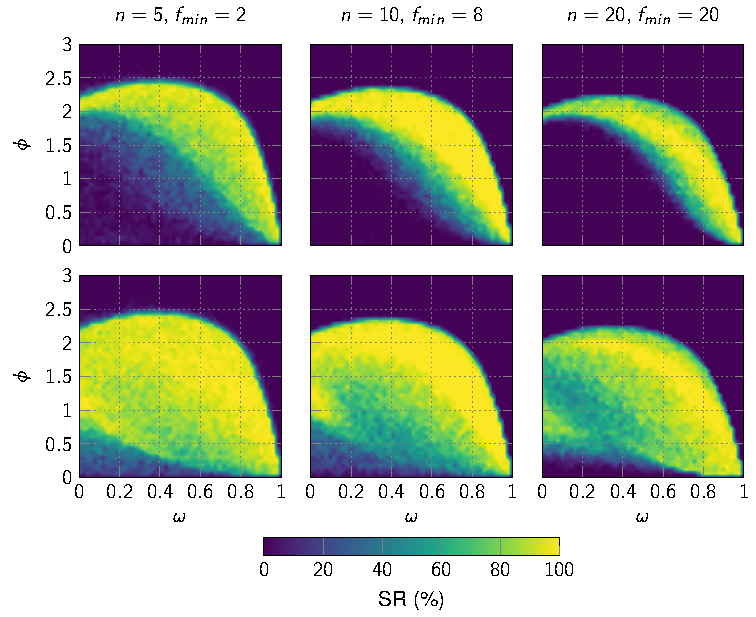
\includegraphics[scale = 1.25]{\thefigures/sensitivity_rosenbrock.pdf}
    \caption{Results of the sensitivity analysis to parameters $\omega$ and $\phi$ for PSO (top) and CPSO (bottom) on the Rosenbrock function in 5, 10 and 20~dimensions. The swarm size is set to 5~times the dimension and the goal to achieve is indicated by $f_{min}$.}
    \label{fig:sensana_rosenbrock}
\end{figure}